% ===========================================================================
\section{Results}
\label{sec:results}
% ===========================================================================

\subsection{The sector}

\begin{table}[htbp]
\centering
\footnotesize
\begin{tabular}{@{}llrr@{}}
\toprule
\textbf{Category} & \textbf{IPCC} & \textbf{Mt \COe{}} & \textbf{$\pm$\%} \\
\midrule
Electricity and heat production & 1A1a & 40.040 & 10.9 \\
Captive gas self-generation     & 1A2  &  5.549 & 15.2 \\
\midrule
\textbf{Total}                  &      & \textbf{45.590} & \textbf{9.7} \\
\bottomrule
\end{tabular}
\caption{Electricity generation, both categories on FY2023--24. The uncertainty column is
Approach~1 per category and for the sector, with the four grid fuel rows' activity errors
treated as fully correlated through the shared TOE conversion (independently they would
give \SI{7.3}{\percent}); the one-sided questions---the coal conversion, the TOE basis,
K-Electric coverage---are structural cases in Table~\ref{tab:scenarios}, not width in
this column.}
\label{tab:results}
\end{table}

\begin{figure}[htbp]
\centering
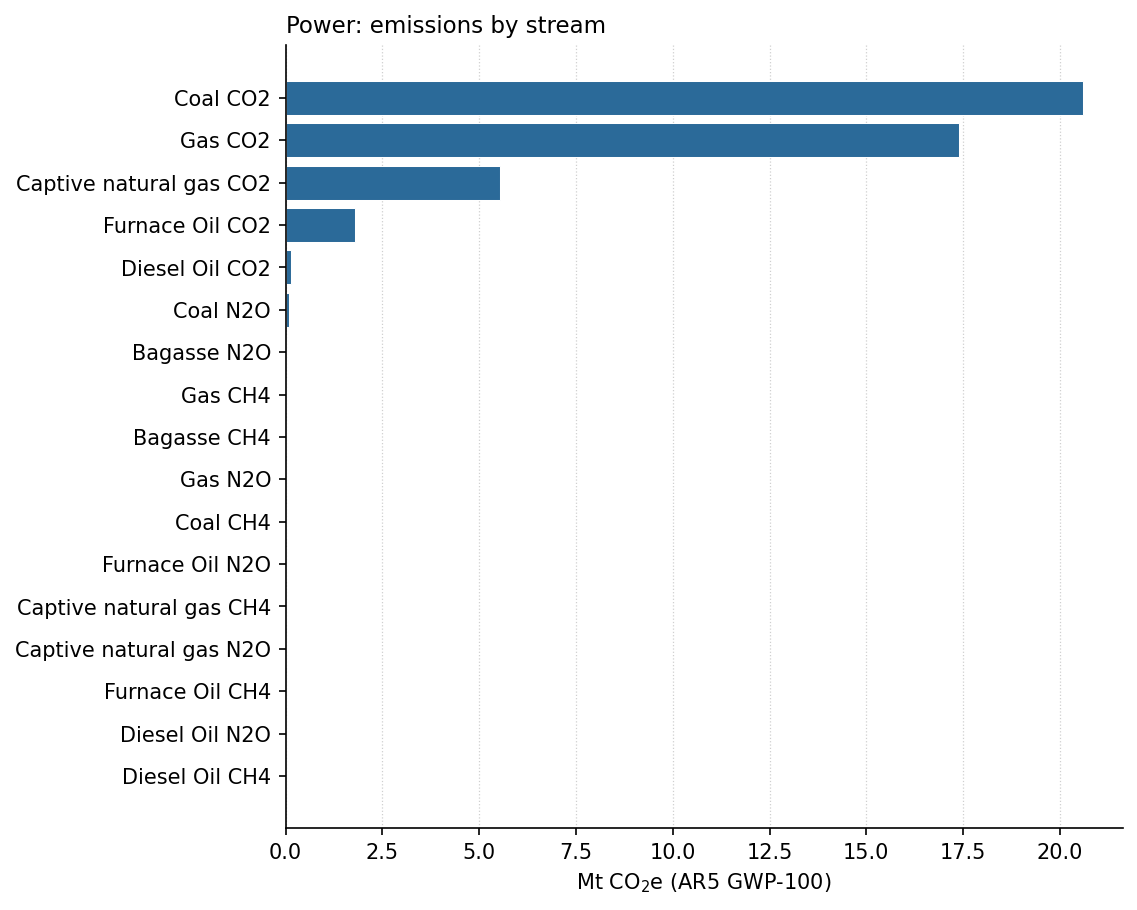
\includegraphics[width=\linewidth]{power_streams.png}
\caption{Emissions by fuel and gas. The sector is \SI{99.6}{\percent} \COtwo{}: the utility
\CHfour{} and \NtwoO{} factors in Table~2.2 are small precisely because large boilers burn
completely.}
\label{fig:streams}
\end{figure}

Coal is \SI{20.59}{\mega\tonne} of \COtwo{}, gas \SI{17.40}{\mega\tonne}, furnace oil
\SI{1.79}{\mega\tonne} and diesel \SI{0.13}{\mega\tonne}. Coal is \SI{37.9}{\percent} of the
energy and \SI{51}{\percent} of the grid emissions, which is the carbon-intensity difference
between coal and gas expressing itself directly---and the reason a fleet shifting between them
moves emissions faster than it moves generation.

The grid category now carries the sector's smallest stream and its first memo item. Eight
sugar-mill cogeneration plants sold \SI{726.85}{GWh} of bagasse-fired electricity to the
grid in FY2023--24 (Table~8's E3 block, reconciled against its printed total); at IPCC
biomass factors that is \SI{0.02}{\mega\tonne} of \CHfour{} and \NtwoO{}---the one
non-fossil methane in the sector, at AR5~28---and \SI{1.09}{\mega\tonne} of biogenic
\COtwo{} reported as a memo outside every total, the carbon having been fixed by the same
season's cane. The activity is generation times an assumed \SI{15000}{\kilo\joule\per\kilo\watt\hour}
heat rate, the sector's one generation-derived stream, and it is labelled structurally
weaker than the metered-fuel streams for exactly that reason. Three plants list biomass and
one lists furnace oil as its alternate fuel; no source read here publishes the co-firing
share, so the furnace-oil caveat is named rather than split.

\subsection{Sensitivities}

\begin{table}[htbp]
\centering
\footnotesize
\setlength{\tabcolsep}{4pt}
\begin{tabular}{@{}p{0.32\linewidth}rp{0.36\linewidth}@{}}
\toprule
\textbf{Case} & \textbf{Mt \COe{}} & \textbf{What it bounds} \\
\midrule
All coal bituminous & 38.995 & lower bound, grid \\
Reported (79\% lignite) & 40.040 & \\
All coal lignite    & 40.318 & upper bound, grid \\
Coal at implied CVs & 38.452 & the conversion question, grid (Sec.~\ref{sec:impliedcv}) \\
Table 3 published energy & 57.820 & legacy published control, grid \\
\midrule
Captive at 900 Btu/scf & 4.995 & lower bound, 1A2 \\
Reported (1000 Btu/scf) & 5.549 & \\
\bottomrule
\end{tabular}
\caption{Both published assumptions, bounded. The coal blend spans \SI{1.32}{\mega\tonne} on
the family reference \SI{40.04}{} (alternatives 38.45 heat-rate, 44.05 with K-Electric,
57.82 legacy control); the gas heating value spans \SI{0.55}{\mega\tonne} on \SI{5.55}{}.
The last row is the aggregate fuel control booked before the coal re-base, kept here so the
blend span and the account change are not read as one quantity.}
\label{tab:sensitivity}
\end{table}

\begin{figure}[htbp]
\centering
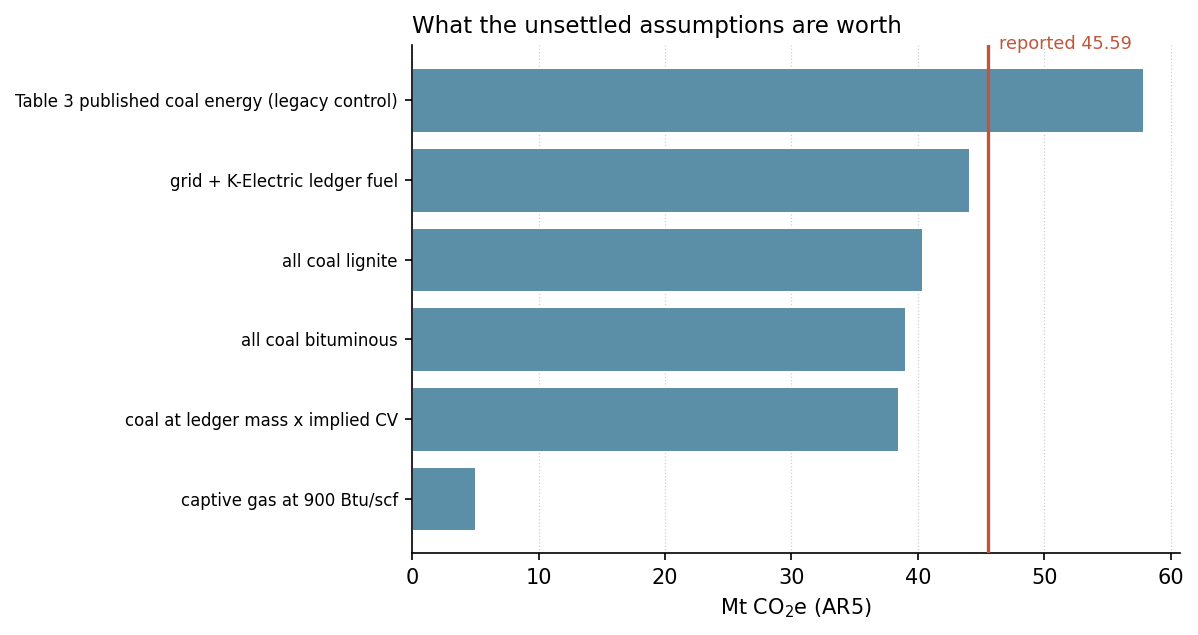
\includegraphics[width=\linewidth]{power_sensitivity.png}
\caption{The same as a range around the reported figure.}
\label{fig:sensitivity}
\end{figure}

Neither span is large relative to the sector, and that is the result. On a mass basis the coal
row alone would span roughly a factor of two; on an energy basis it spans
\SI{3.3}{\percent} of the grid category. The account change is a separate and larger matter
and is kept separate: the legacy control sits \SI{17.78}{\mega\tonne} above the reference,
which is \num{13} times the blend span, and no reading of the blend reaches it.

\begin{table}[htbp]
\centering
\footnotesize
\begin{tabular}{@{}lrrr@{}}
\toprule
\textbf{Structural case} & \textbf{Mt \COe{}} & \textbf{P2.5} & \textbf{P97.5} \\
\midrule
Reference (family reference)  & 40.040 & 36.0 & 44.5 \\
All coal bituminous           & 38.995 & 34.9 & 43.4 \\
All coal lignite              & 40.318 & 36.1 & 44.9 \\
Coal at implied CVs           & 38.452 & 34.4 & 42.9 \\
Table 3 published energy      & 57.820 & 51.8 & 64.3 \\
TOE on a gross basis          & 37.168 & 33.3 & 41.4 \\
Grid + K-Electric ledger fuel & 44.054 & 39.8 & 48.5 \\
\midrule
Captive at 900 Btu/scf        &  4.995 &  4.3 &  5.8 \\
\bottomrule
\end{tabular}
\caption{The one-sided questions as named cases, each with a conditional parametric
interval and no structural probability. Discrete choices are kept unsampled so a
confidence interval cannot conceal a boundary or coverage choice; the parametric
$\pm$\SI{10.9}{\percent} above is conditional on the reference configuration of every row
in this table.}
\label{tab:scenarios}
\end{table}

\subsection{Provincial allocation, corrected}

\begin{figure}[htbp]
\centering
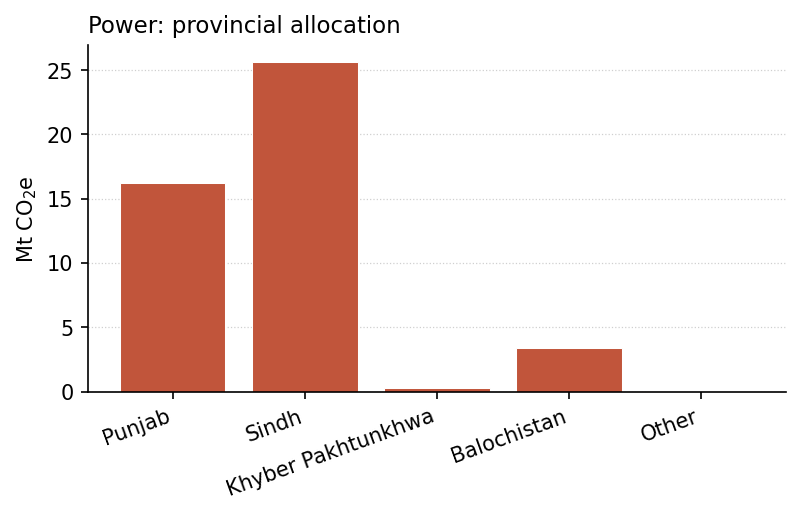
\includegraphics[width=\linewidth]{power_provincial.png}
\caption{Punjab \SI{16.24}{\mega\tonne}, Sindh \SI{25.67}{\mega\tonne}, Balochistan
\SI{3.41}{\mega\tonne}, Khyber Pakhtunkhwa \SI{0.27}{\mega\tonne}. Unlike almost every other
sector in this inventory, the ordering does not follow population, because it follows the
plants---and above all the Thar coalfield.}
\label{fig:provincial}
\end{figure}

This geography has now been corrected twice, each time by a better class of evidence, and
the second correction is larger than the first. The original capacity proxy gave Khyber
Pakhtunkhwa \SI{14.24}{\percent} of a combustion sector whose electricity there is hydro;
plant-wise generation moved \SI{6.2}{\mega\tonne} out of that province. But the generation
proxy still blended all fuels onto one share, and the ledger joined to the report's own
plant-location table (Table~5) shows the fuels do not share a geography: coal is
\SI{89}{\percent} Sindh on the stations' booked energy (four Thar mine-mouth plants, Port Qasim and
Lucky against Sahiwal alone in Punjab), the RLNG combined-cycle corridor is Punjab, the
pipeline-gas plants sit on the Sindh and Balochistan fields, and the furnace oil actually
burned in FY2023--24 is entirely Punjab---Hub, the Balochistan plant that dominated older
vintages of this split, reports zero fuel for the year. Allocating each fuel on its own
plants moves \SI{12.6}{\mega\tonne} from Punjab to Sindh at an unchanged national total
and makes Sindh, not Punjab, the sector's dominant province. Each per-fuel share is
recomputed from the ledger by a test, so the committed geography cannot quietly outlive
its derivation; the energy weights carry their evidence classes (MMBTU exact, volumes at
the declared heating value, coal mass at the per-plant implied calorific values of
Section~\ref{sec:impliedcv}). \ref{app:provincial} records the replaced proxies.

\subsection{Contribution to the national inventory}

\begin{table}[htbp]
\centering
\footnotesize
\begin{tabular}{@{}lrr@{}}
\toprule
\textbf{Category} & \textbf{Level (\%)} & \textbf{Variance (\%)} \\
\midrule
Electricity and heat production & 9.00 & 0.80 \\
Captive gas self-generation (1A2)        &  1.25 & 0.03 \\
\bottomrule
\end{tabular}
\caption{Shares of the national total and of national Approach-1 variance.}
\label{tab:keycat}
\end{table}

Grid generation is the third largest category in Pakistan and---since the uncertainty
rebuild---no longer a large contributor to national variance: \SI{0.80}{\percent}, down
from a published \SI{3.24}{}, and from an earlier vintage in which it ranked second after
enteric fermentation. The fall is not new information about the fleet; it is the flat
activity percentage being replaced by per-fuel widths the evidence supports, and the
questions actually worth megatonnes---the coal conversion, the TOE basis, K-Electric
coverage---moving to the structural-scenario table where a probability interval cannot
conceal them. The honest summary is that this sector's parametric uncertainty is modest
and its structural uncertainty is large, one-sided and named.

Captive gas self-generation contributes \SI{0.03}{\percent} of national variance, which is the expected
result for a category whose activity is metered and whose factor is an IPCC default: its
\SI{15.2}{\percent} band is small and its size is modest. Its value to the inventory is not
uncertainty reduction but coverage---it is the first number inside a gap that was previously
empty.
